\documentclass[epsfig]{article}
\usepackage{epsfig}
\usepackage{amsmath}
\usepackage{verbatim}
\usepackage{booktabs}
\usepackage{subfig}
\usepackage{graphicx}
\usepackage{multirow}
\usepackage{epsfig}
\usepackage{amsmath}
\usepackage{graphicx}
\usepackage{subfig}
\usepackage[english]{babel}
\usepackage{rotating}
\usepackage{multirow}
\usepackage[english]{babel}
\textwidth 6.7in
\oddsidemargin -0.1in
\textheight 8.50in
\topmargin -0.55in
\renewcommand{\textfraction}{0.25}
\renewcommand{\floatpagefraction}{0.7}
\begin{document}
\parindent=0pt
\author{Kentaro Hoffman}
\title{COMP/ELEC/STAT 502 HW 05}
\maketitle

  
 \subsection*{Question 2a}
 \begin{table}[htbp] 
\center
\caption{Parameters for Question 2a}
  \label{tab:NP}
  %\scalebox{0.9}{ % You can scale the size of the table by changing this number
   \scalebox{1.0}{
   \begin{tabular}{p{6cm} p{.05cm} p{8cm}}
\toprule
  \multicolumn{3}{l}{\bf Network parameters} \\
\bottomrule \noalign{\smallskip}
  Topology & & 64 PEs in a 8x8 grid centered at (3.5, 3.5)  \\
\toprule
  \multicolumn{3}{l}{\bf Learning parameters} \\
\bottomrule \noalign{\smallskip}
  Initial weights & & drawn from (U[3, 4], U[3, 4]) \\
  Initial Learning rate (a(0)) & & 0.5\\
  Initial Standard Deviation of the Neighborhood Function ($\sigma$(0)) & & 7\\
  Decay term for Neighborhood  ($\alpha$) && 20,000\\
  Decay term for Learning Rate  ($\beta$) && 5,000\\
  Number of Learning Steps  & & 78,000\\
  
  \\\toprule
 \multicolumn{3}{l}{\bf Input / output data, representation, scaling} \\
\bottomrule \noalign{\smallskip}
Data && 4000 data points equally distributed with a standard Normal distribution about (0,0), (7,0), (0,7), (7,7)\\
%  %\# learn steps performed & & 180,365 (error threshold reached)\\

 \bottomrule \noalign{\smallskip}
   \end{tabular}
   } 
\end{table}
\textbf{Explanation of Decay Terms $\alpha$ and $\beta$}\\
\newline
In an SOM, typically no convergence will occour unless there is a Learning Rate and a Neighborhood Function that decays with time. The Learning rate is based off of a step function and the Neighborhood function is based off of the gaussian where every $\alpha$ or $\beta$ learning steps, the parameter is decreased in the following fashion:\\
\textbf{Learning Rate}\\
Every $\alpha$ learning steps, 
$$a(t+1) = a(t) /  1.2$$
\textbf{Neighborhood Function}\\
Every $\beta$ steps:
$$\sigma(t+1) =  \sigma(t)/  1.5$$ 
$$h_{j, c(x)} (t+1) = exp({\frac{-(c(x)-j)^2}{\sigma(t+1) ^2}})$$ 
Where $h_{j, c(x)}$ is the neighborhood function for the node j when c(x) is the winner of the current learning step.\\
\newline
\newline
\textbf{Weight Updating Scheme}\\
As for the weight updating scheme, it is the same as the one described in class:\\
Randomly choose a datapoint x, the weights for node j at time t+1 is\\
$$w_j(t+1) =  w_j(t)  + a(t) h_{j, c(x)} (t) ( x- w_j(t))$$ 

\subsection*{Results}
Overall, the SOM does a good job at  identifying the 4 clusters. 
\begin{center}
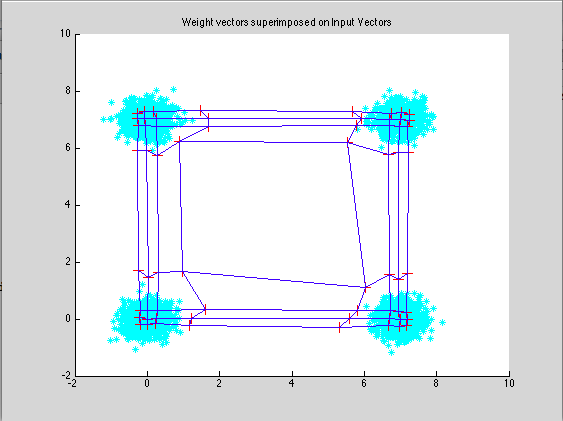
\includegraphics[scale=0.42]{pic1}
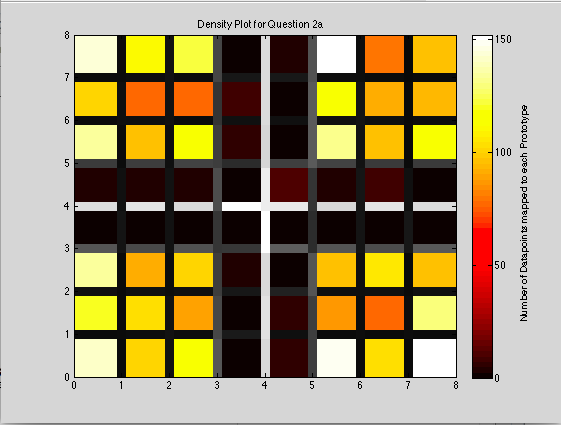
\includegraphics[scale=0.42]{pic2}
\end{center}
\textbf{(left)} A graph of the datapoints (cyan) and the prototypes (red). \textbf{(right)} A U-matrix of the simulation on the right. Where the color of each cell represents the number of datapoints mapped to each prototype and the color of the line represents the euclidean distance between two prototypes with a white line indicating a large difference and a black line representing a small difference.\\
\newline
As you can see in the plot to the right, the prototypes are slighly wonkey at the corners but are still generally clustered as one would expect them--with large culsters in the datapoints and a sparse number of them in the areas between the clusters. Moreover, the wellness of this simulation can be seen in the U-matrix for the SOM on the left.\\
\newline
The image on the right is an illustration of how many datapoints are mapped to each protype. So the first protype, (0,0) is the lower left PE and it has a good number (around 130) of datapoints mapped to it as it is in the middle of a cluster. What is most interesting to note however is the large black cross. This cross indicates that there are a set of PE such that hardly any datapoints are mapped to them. Or in other words, these prototypes are "dead PEs". Using these "dead PEs", and the large white "wall" between the populated groups, one can see that 4 very distinct regions have been recognized successfully.\\
\newpage
\section*{Question 2b}
 \begin{table}[htbp] 
\center
\caption{Parameters for Question 2a}
  \label{tab:NP}
  %\scalebox{0.9}{ % You can scale the size of the table by changing this number
   \scalebox{1.0}{
   \begin{tabular}{p{6cm} p{.05cm} p{8cm}}
\toprule
  \multicolumn{3}{l}{\bf Network parameters} \\
\bottomrule \noalign{\smallskip}
  Topology & & 10 PEs in a 10x10 grid centered at (3.5, 3.5)  \\
\toprule
  \multicolumn{3}{l}{\bf Learning parameters} \\
\bottomrule \noalign{\smallskip}
  Initial weights & & drawn from (U[3, 4], U[3, 4], U[3,4]) \\
  Initial Learning rate (a(0)) & & 0.2\\
  Initial Standard Deviation of the Neighborhood Function ($\sigma$(0)) & & 3\\
  Decay term for Neighborhood  ($\alpha$) && 10,000\\
  Decay term for Learning Rate  ($\beta$) && 4,000\\
  Number of Learning Steps  & & 198,000\\
  
  \\\toprule
 \multicolumn{3}{l}{\bf Input / output data, representation, scaling} \\
\bottomrule \noalign{\smallskip}
Data && 4000 data points equally distributed with a standard Normal distribution about (0,0,0), (7,0,0), (0,7,0), (7,7,0)\\
%  %\# learn steps performed & & 180,365 (error threshold reached)\\

 \bottomrule \noalign{\smallskip}
   \end{tabular}
   } 
\end{table}

\section*{Results}

\begin{center}
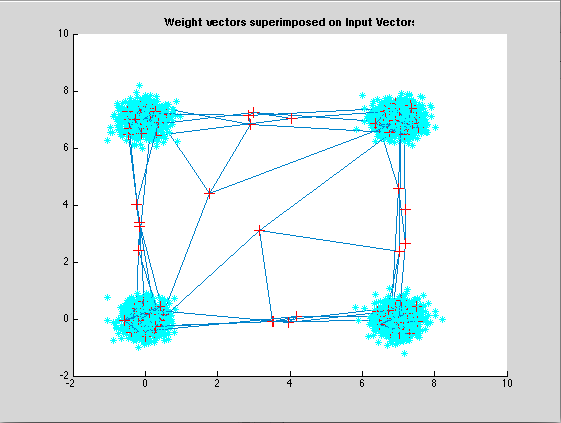
\includegraphics[scale=0.42]{pic3}
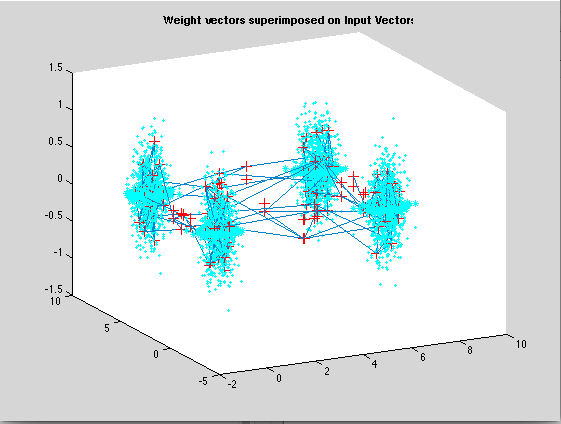
\includegraphics[scale=0.42]{pic4}
\end{center}
\textbf{Caption:} (left) A view of the prototypes superimposed on the datapoints. (right) A shot of the same figure from an isometric perspective\\
\newline
From the plots above, we can see that the SOM has done a good job learning the 3 dimensional data. The view from the top shows that it manages to converge to a similar figure as the previous question, and the isometric view of the right shows that the weights, even though they were initialized in 2-D were able to spread out into the z axis and understand the 3 dimensionalality of the new data. The one issue in this is that the convergence is not very clean and two points in the plot on the left are shown to be fairly close to the center compared to all of the other points. This brings up issues in the plot below.
\begin{center}
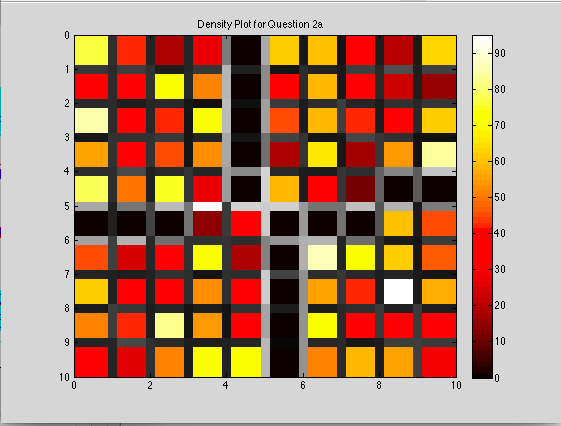
\includegraphics[scale=0.6]{pic6}
\end{center}
In this density plot, we can see about what we would expect, that the SOM has divided the grid up into 4 sections and deivded those sections by a line of no "dead" PEs, or PE that are not the winner for any datapoint. Moreover the regions of dead PEs are correspond with white fenses indicating a large euclidean distance between the points, a sign of a difference beteween clusters. The one issue that can be seen are the two green points in the middle. These are the two problematic points that were close to the center that were mentioned above. And unfortunately, the density plot is showing that this SOM might not be a good as it immediatly seems as the density plot shows the row of "dead PE" is not straight like in the previous part, but misaligned. The misalignment comes from the fact that there are two PEs close to the center but their neighbors are not. But still, since it is possible to still delineate the 4 groups from each other, it seems like the SOM has not done a bad job at understanding the data.
\newpage
\section*{Question 3}
To illustrate the clustering relations in another form, a modified U-Matrix was created. 
\begin{center}
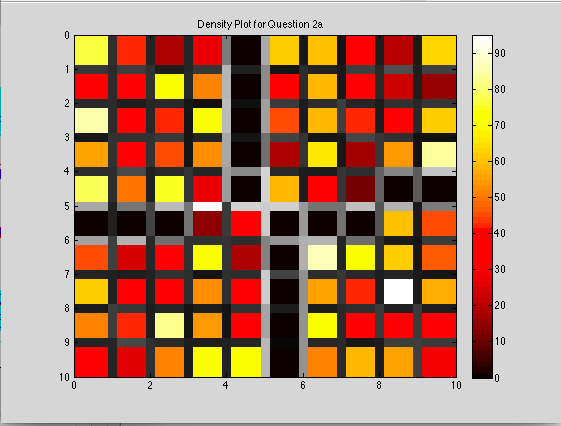
\includegraphics[scale=0.6]{pic6}
\end{center}
Like in the previous quesiton, one can see that the blue colored blocks are the "dead" PEs that indicate PEs that were not winners for any datapoint. But in addition, the newly added lines also gives us valuable information. The whiter the line, the larger the euclidean difference between the weights of the two nodes there is. And if one notices that the white lines tend to follow the black squares, we can safely say that the 4 distict regions are those that are delineated by the black squares.
\newpage
\section*{Question 4}
\begin{table}[htbp] 
\center
\caption{Parameters for Question 2a}
  \label{tab:NP}
  %\scalebox{0.9}{ % You can scale the size of the table by changing this number
   \scalebox{1.0}{
   \begin{tabular}{p{4cm} p{.05cm} p{8cm}}
\toprule
  \multicolumn{3}{l}{\bf Network parameters} \\
\bottomrule \noalign{\smallskip}
  Topology & & 100 PEs in a 10x10 grid centered at (0, 0)  \\
\toprule
  \multicolumn{3}{l}{\bf Learning parameters} \\
\bottomrule \noalign{\smallskip}
  Initial weights & & drawn from U[0, 0] \\
  Learning rate (L(t)) & & 0.25\\
  Neighborhood Function & & 5\\
  Neighborhood 
  Decay term for Neighborhood  ($\alpha$) && 5,000\\
  Decay term for Learning Rate  ($\beta$) && 5,000\\
  Number of Learning Steps  & & 30,000\\
  
  \\\toprule
 \multicolumn{3}{l}{\bf Input / output data, representation, scaling} \\
\bottomrule \noalign{\smallskip}
Data && 125, 4 dimensional datapoints that represent the physical characters of the 3 classes of flowers in the iris dataset. \\
%  %\# learn steps performed & & 180,365 (error threshold reached)\\

 \bottomrule \noalign{\smallskip}
   \end{tabular}
   } 
\end{table}
\newpage
\section*{Learning Proscess}
\begin{center}
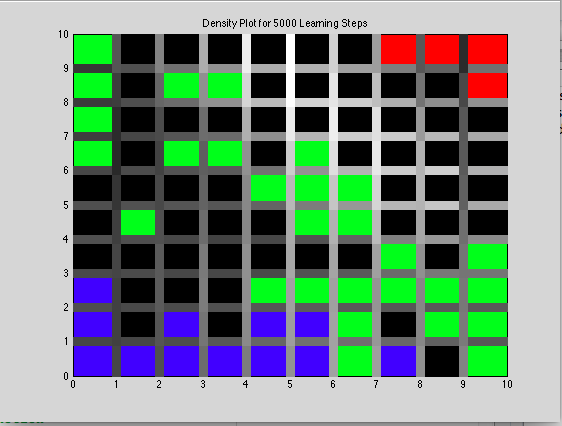
\includegraphics[scale=0.4]{pic62}
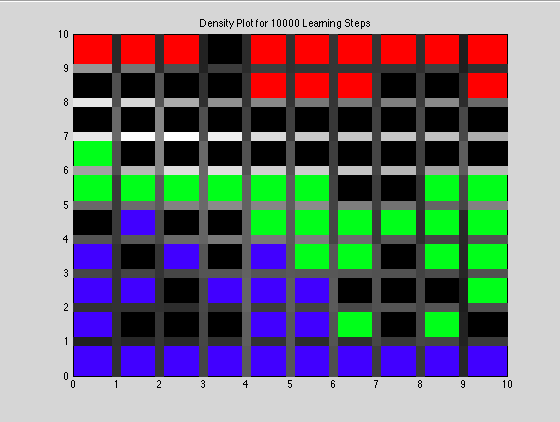
\includegraphics[scale=0.4]{pic63}
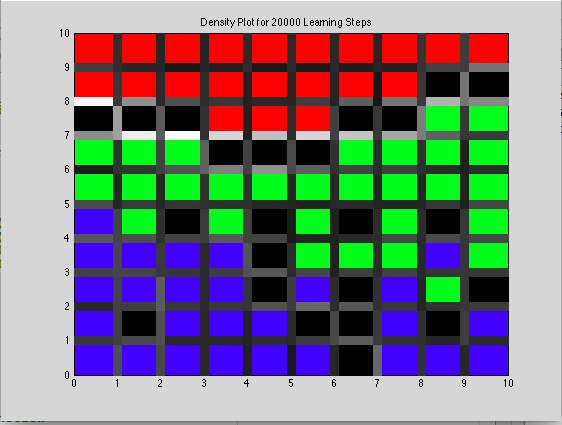
\includegraphics[scale=0.4]{pic64}
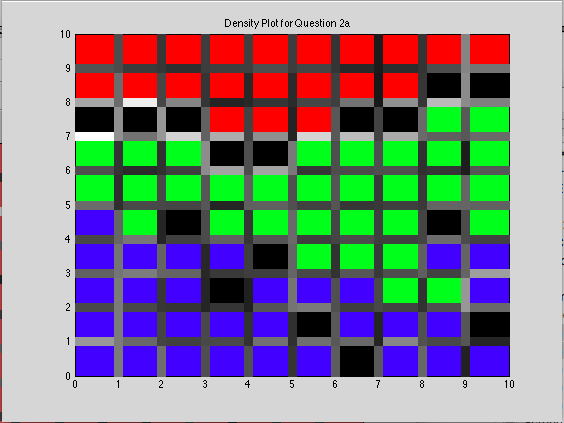
\includegraphics[scale=0.4]{pic61}
\end{center}
\textbf{Top left} SOM grid at 5000 learning steps. \textbf{(Top right)} SOM grid at 10,000 learning steps, \textbf{(bottom left)} SOM grid at 20,000 steps \textbf{(bottom right)} SOM grid at the final convergence time of 30,000 steps. If it is red, then Setosa was the most common, green is Versacolor and blue is Virginica and if the PE is dead, then black\\
\newline
As we can see from the plots above, the SOM seems to be learning the data quite well. In the begining it has quite the bit of trouble as there are hardly any Setosa flowers even though they represent a 1/3 of the data points and the white walls do not lign up with the black dead regions. At the 10,000 mark, the SOM starts to resemble the finish product and the walls start to appear in the right locations but things are not truly finished till the number of Setosa, Versacolor, and Virginicia take up about equal numbers of PEs. And this finally occours when the SOM hits the final number of 30,000 learning steps. 
\section*{Results}
\begin{center}
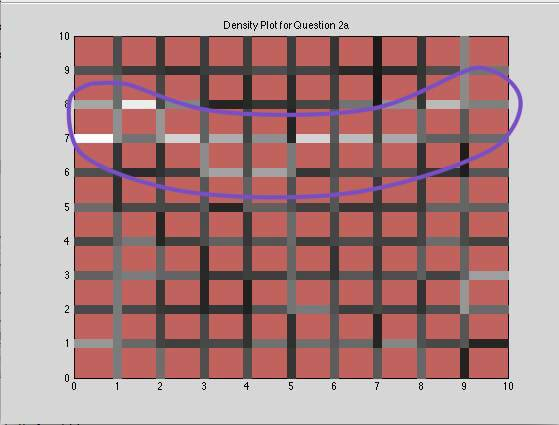
\includegraphics[scale=0.5]{pic7}
\end{center}
In the picture above, we see the Modified U-matrix for the SOM. More interestingly, the purple hotdog shaped  region indicates that there is a large euclidean difference between the points at the top of the grid as compared to those at the bottom. This seems to hint that possibly there is a type of flower, most likely Setosa as the perceptrons never had any problems classifying this flower, that is very different in phyical dimensions from the rest of the flowers. Moreover, the lack of boundries in the rest of the dataset is also quite telling as it would indicate that the other two flowers, Versacolor and Virginica are hard to distinguish from one other. Which would in turn explain the errors that the Perceptrons had in classifying the two apart.

\begin{center}
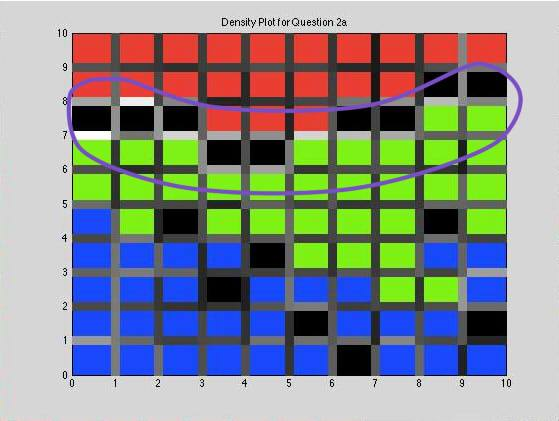
\includegraphics[scale=0.5]{pic8}
\end{center}
To confirm this hypothesis, for each prototype, I found the most common type of flower that that is associated with each protype and then colorcoded the cell. If it is red, then Setosa was the most common, green is Versacolor and blue is Virginica. And this plot perfectly confirms my hypothesis. Setosa is very different from the other flowers as it is seperated by a high fense while the lack of fenses between Versacolor and Virginica seems to indicate that the physical difference between the two groups of flowers is slight, a fact that explains the trouble the Perceptrons had in classifying the two.
\end{document}


